\chapter{システムを用いた実験,評価}

\section{まえがき}
ここでは,観測者であるTWELITE CUEタグの位置の推定を目指し,第\ref{chap3}章において評価したシステムを用いて簡単な実験を実施した.
その実験の結果と評価についてまとめる.

\section{実験の概要}

\subsection{測定機器}
先述のTWELITE CUE,MONOSTICKのほかに,サブスクライバPCとしてMQTTブローカーMosquittoを導入済みのWindows PC1台,
MQTTプロトコル(TCP/IP)を実現するためのWi-Fiルーター1台を用いて行った.


\subsection{実験環境}
図\ref{TWjikken}に実験環境の写真を示した.
室内で180cm四方の机を囲むような環境になっているが,机を用いたのはMONOSTICKについて,床から離して設置するよう推奨されているためである.
MONOSTICKを取り付けたマイコン(Raspberry Pi)は机の四隅に設置されている.
同様に床から離すよう推奨されているTWELITE CUEタグは,自由に動くプラスチック製のワゴンに置かれ,そこから発信されたデータは4か所のMONOSTICK・MQTTプロトコルを介してサブスクライバPCに集約されるようになっている.


\begin{figure}[htb]
  \centering
   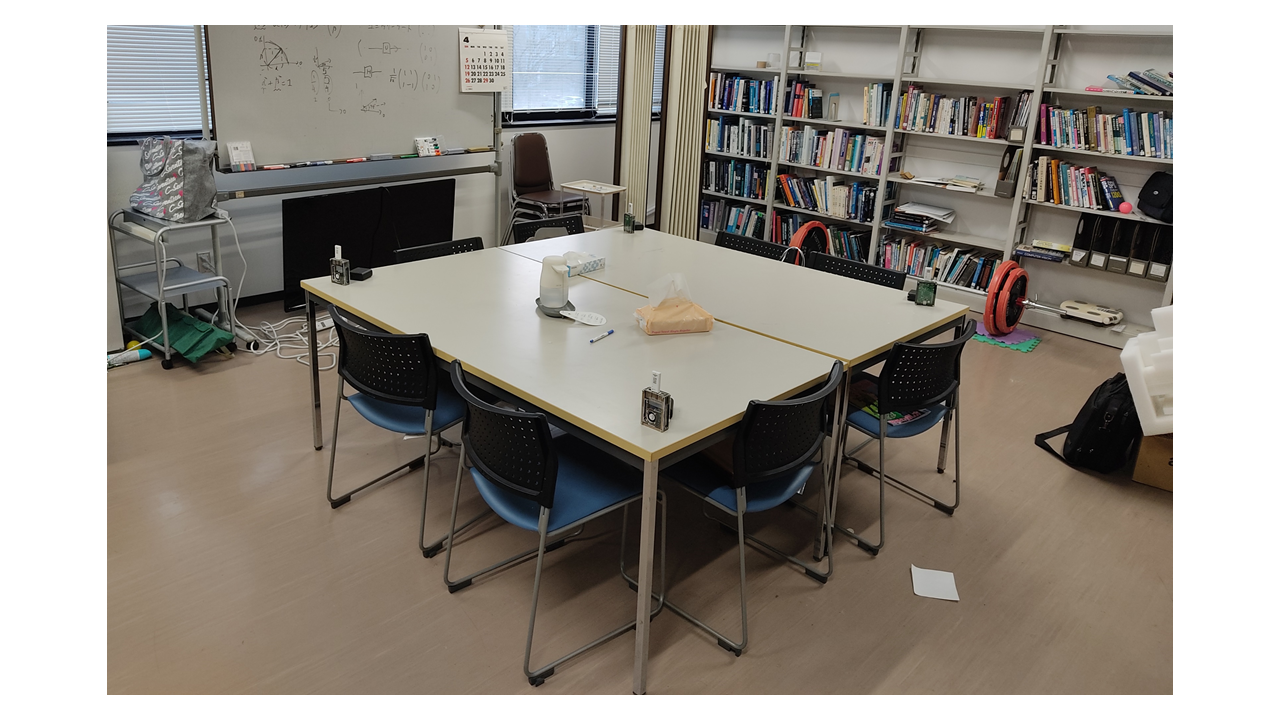
\includegraphics[width = 15cm, bb= 0 0 1000 600]{chapter4/TWjikken.png}
   \caption{実験環境の写真}
   \label{TWjikken}
\end{figure}


\subsection{実験方法}

\begin{enumerate}
  \item 机の四隅に置かれたMONOSTICK・Raspberry PiからサブスクライバPCにMQTTでデータが送られるよう設定する.
  \item 1.56Hz(加速度サンプリング頻度25Hz,送信サンプル数16)でデータを送信するよう設定したTWELITE CUEタグを置いたプラスチックワゴンを机を回るように自由に移動させる.
  移動の様子は同時にビデオ撮影を行って記録しておく.
  \item サブスクライバPCで,集約されたデータに線形補間による補間と状態空間モデルによるフィルタリングを行ったのち比較を行い,観測者から一番近いMONOSTICKが4台のうちどれであるか求める.
  \item ビデオ撮影によって得られた情報と比較を行い,今回のシステムによる推定の正解率を調べる.
\end{enumerate}


\section{実験結果}
実験中192回のデータ送信があったうち,システムによって得られた推定の正解は174回であり,正解率は90.6\%であった.
不正解となった約10\%のデータは約5秒程度の連続した不正解であった.

\section{実験の評価}
システムによる推定の正解率が高く,システムの近距離の判別性能は高いといえる.
不正解となった時間について,その時間はどのMONOSTICKにも極度に接近していない状態であった.
そのため,不正解の一因としては,最も近いタグとそれ以外のタグとの距離比があまりないために電波強度に差が生まれず,システムが推定を誤ったと考えられる.











